\documentclass{article}
\documentclass[12pt, french]{report}
\usepackage[utf8]{inputenc}
\usepackage[T1]{fontenc}
\usepackage[french]{babel}

\usepackage{algorithm}
\usepackage{amsthm}
\usepackage{amsfonts}
\usepackage{hyperref}
\usepackage{graphicx}
\usepackage{amsmath}
\DeclareMathOperator*{\argmax}{arg\,max}
\DeclareMathOperator*{\argmin}{arg\,min}

\newtheorem{definition}{Définition}
\newtheorem{remark}{Remarque}
\newtheorem{example}{Exemple}
\newcommand{\floor}[1]{\lfloor #1 \rfloor}


\begin{document}
\thispagestyle{empty}
\setlength\headheight{0pt} 
\begin{center}
\begin{center}

\includegraphics[width=0.45\linewidth]{montpellier.png}     
\end{center}	

        \vspace{0.40cm}
        {\scshape\LARGE Université de Montpellier, France\par}
        \vspace{0.50cm}
        {\scshape\Large Projet HMMA307 - M2 MIND \par}
        \vspace{0.90cm}

        {\Large\bfseries Utilisation de la médiane géométrique  et de l'estimation robuste dans des espaces de Banach\par}
        
        \vspace{1cm}
        {\Large\itshape Hanna Bacave\par}
        \vspace{0.70cm}


\begin{center}
    Novembre 2020
\end{center}

\end{center}

\newpage

\renewcommand{\contentsname}{Table des matières} 
\tableofcontents
\pagebreak
\addcontentsline{toc}{section}{Introduction}


\section*{Introduction}
Dans ce document, nous allons présenter la façon dont nous avons implémenté, grâce au logiciel Python, les travaux effectués par Stanislav Minsker \textit{\href{https://arxiv.org/pdf/1308.1334.pdf}{Geometric median and robust estimation in Banach spaces}} [0]. Après une rapide présentation de ce qu'est l'estimateur médian, nous nous interesserons plus particulièrement aux travaux de Stanislav Minsker, avant de réaliser l'implémentation de ces recherches.

\vspace{0.5cm}

\section{Présentation de la régression quantile}
\vspace{0.2cm}
\subsection{Médiane}
A partir de la ressource [1], nous allons introduire la définition de la médiane. 
\vspace{0.1cm}
\begin{definition}
Soit $y_1, ..., y_n \in \mathbb{R}$, on définit la \textit{médiane} par :
$$Med_{n}(y_1, ..., y_n) \in \argmin_{\mu \in \mathbb{R}} \frac{1}{n} \sum\limits_{i=1}^{n} | y_i - \mu |.$$
\end{definition}
\vspace{0.1cm}
En pratique, on utilise plutôt une écriture de la médiane comme suit : 
$$Med_{n}(y_1, ..., y_n) =
\begin{cases}
y_{\floor{\frac{n}{2}}-1} \ si \ n \ est \ pair \\
\frac{y_\floor{\frac{n}{2}} + y_{\floor{\frac{n}{2}}-1}}{2} \ si \ n \ est \ impair
\end{cases}
.
$$
\vspace{0.2cm}
\subsection{Quantile}
A partir de la ressource [1], nous allons introduire la définition du quantile. 
\vspace{0.1cm}
\begin{definition}
Le \textit{quantile de niveau $\alpha$} est défini par :
$$\forall \alpha \in ]0, 1], \ q_{\alpha}(y_1, ..., y_n) = \inf \{t \in \mathbb{R} : F_n(t) \geq \alpha \}.$$
où
$$F_n(t) = \frac{1}{n} \sum\limits_{i=1}^{n}\mathbb{1}_{\{y_i \leq t \}}.$$
\end{definition}
\vspace{0.1cm}
\begin{remark} 
Le quantile de niveau $\alpha = 0.5$ est la médiane.
\end{remark}
\vspace{0.1cm}
\begin{definition}
On définit la \textit{fonction de perte de niveau $\alpha$} par :
$$l_\alpha : 
\begin{array}{l rcl}
 & \mathbb{R} & \longrightarrow & \mathbb{R} \\
    & x & \longmapsto &  \begin{cases}
-(1 - \alpha)x \ si \ x \geq 0 \\
\alpha x \ si \ x \leq 0
\end{cases}
.
\end{array}
$$
\end{definition}
\vspace{0.2cm}
\subsection{Régression quantile}
On dispose de 
\begin{itemize}
    \item $y_1, ..., y_n \in \mathbb{R}$ observations,
    \item $x_1, ..., x_n \in \mathbb{R}^p$ variables explicatives.
\end{itemize}
\vspace{0.1cm}
\begin{definition}
Soit $\alpha \in ]0,1[$, on appelle \textit{régression quantile} les coefficients :
$$\beta^{\alpha} \in \argmin\limits_{\beta \in \mathbb{R}^p} \frac{1}{n} \sum\limits_{i=1}^{n} l_{\alpha}(y_i - x_i^T\beta),$$
où 
$$X = \begin{pmatrix}
x_1^T \\
x_2^T \\
\vdots\\
x_n^T
\end{pmatrix} 
\in \mathbb{R}^{nxp}.$$
\end{definition}
\vspace{0.1cm}
\begin{remark}
La régression quantile est efficace sur des jeux de données : 
\begin{itemize}
    \item ayant une distribution non symétrique par rapport à la moyenne
    \item ayant une nature hétéroscédastique.
\end{itemize}
En fait, la régression quantile est moins sensible aux points aberrants que d'autre régression.
\end{remark}
\vspace{0.1cm}
\begin{example}
Après avoir simulé des données dont la représentation est non symétrique par rapport à la moyenne et portant des points abérrants, nous allons comparer la régression médiane avec une régression linéaire présentée dans la Figure 1. 
 \begin{figure}[!h]
    \begin{center}
   \caption{\label{étiquette} Comparaison de la régression linéaire avec la régression quantile sur un jeu de données simples}
   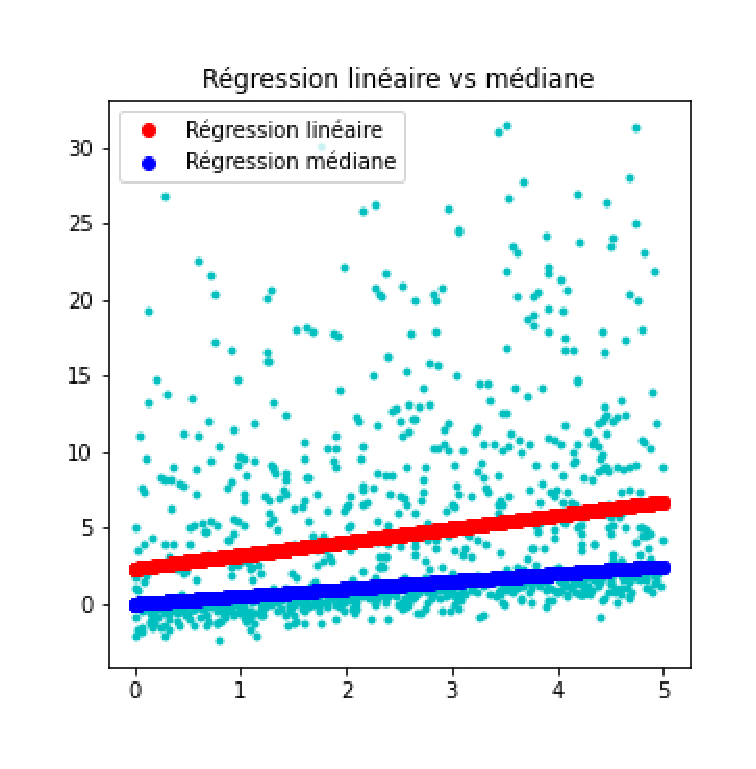
\includegraphics[width=8cm]{reg1.pdf}
   \end{center}
    \end{figure}
On observe que la régression linéaire accorde plus de poids aux valeurs extrêmes ce qui lui confère un résultat moins efficace que pour la regression quantile. 
\end{example}
\vspace{0.5cm}

\section{Régression quantile en grande dimension avec des données sparses}
Dans cette section, nous allons présenter la façon dont nous avons implémenté la méthode de régression quantile en grande dimension avec des données sparses, présentée dans la ressource [0]. Ensuite, nous présenterons le moyen utilisé pour comparer les régressions entre elles. 
\vspace{0.2cm}
\subsection{Implémentation pratique}
On définit : 
\begin{itemize}
    \item $x_1, ..., x_n \in \mathbb{R}^D$,
    \item $\lambda_0 \in \mathbb{R}^D$.
\end{itemize}
\begin{definition}
On veut résoudre le problème d'optimisation suivant : 
$$Y_j = \lambda_0^T x_j + \epsilon_j$$
où
\begin{itemize}
    \item $\epsilon_j$ est un vecteur iid de moyenne $0$, mais n'est pas gaussien ;
    \item $\lambda_0$ est un vecteur sparse, c'est-à-dire que la dimension s du support de $\lambda_0$ est très nettement inférieure à D ;
    \item $D >> n$
\end{itemize}
\end{definition}
\vspace{0.1cm}
Une première solution serait de calculer l'estimateur Lasso de $\lambda_0$ :
$$\hat{\lambda}_\epsilon = \argmin\limits_{\lambda \in \mathbb{R}^D} \left[ \frac{1}{n} \sum\limits_{j=1}^{n} (Y_j - \lambda^T x_j)^2 + \epsilon \|\lambda\|_1 \right].$$
Or, cette solution n'est pas la plus efficace, car pour augmenter son score, il faudrait changer le modèle. Notre objectif est donc - sans changer le modèle, ni faire de suppositions sur $\epsilon$ - de calculer le meilleur estimateur sur ce type de données. On se propose de procéder comme suit : 
\begin{enumerate}
    \item On commence par définir les quantités suivantes : 
    \begin{itemize}
        \item $t > 0$ fixé, 
        \item $k = \floor{3.5t} + 1$
        \item $m = \floor{\frac{n}{k}}$
    \end{itemize}
    On divise notre échantillon $x_1, ..., x_n$ en $k$ groupes disjoints $G_1, ..., G_k$ de taille $m$ chacun. De plus, pour $1 \leq l \leq k$, on définit $G_l = \{(l-1)m + 1, ..., lm \}$ et 
$$\mathbb{X}_l = (x_{j_1} | ... | x_{j_m}),$$ 
où,  $j_i = (l - 1)m + i \in G_l$.
    \item On calcule ensuite l'estimateur Lasso sur l'ensemble $G_l$, de la façon suivante :
    $$\hat{\lambda}_\epsilon^l = \argmin\limits_{\lambda \in \mathbb{R}^D} \left[ \frac{1}{|G_l|} \sum\limits_{j \in G_l} (Y_j - \lambda^T x_j)^2 + \epsilon \|\lambda\|_1 \right]$$.
    \item Enfin, après avoir calculé tous les estimateurs Lasso pour $1 \leq l \leq k$, on calcule la médiane de toutes les estimations :
    $$\hat{\lambda}_\epsilon^* = med(\hat{\lambda}_\epsilon^1, ..., \hat{\lambda}_\epsilon^k),$$
    où $med()$ désigne la médiane géométrique avec la norme euclidienne sur $\mathbb{R}^D$.
\end{enumerate}
\vspace{0.1cm}
Dans la suite de cette section, nous allons décrire comment nous avons implémenté la stratégie présentée plus haut. \\
Pour commencer, nous avons construit une classe prenant comme paramètres n, D, t et s, où 
\begin{itemize}
    \item n et D sont la taille de l'espace des variables ;
    \item t est la quantité permettant de créer les groupes disjoints $G_1, ..., G_k$ ;
    \item s est la sparcité de $\lambda_0$, cette quantité permet de définir la proportion de valeurs non nulles dans $\lambda_0$, qui est $\frac{s}{D}$.
\end{itemize}
Ensuite, nous avons défini les matrices avec lesquelles nous travaillons : 
\begin{itemize}
    \item La matrice $\mathbb{X}$, de taille (n,D), a été défini à l'aide de la fonction np.random.rand() ;
    \item le vecteur $\epsilon$, de taille (1,n), a été défini à l'aide de la fonction np.random.rand() ;
    \item le vecteur Y, de taille (1,n), a été défini par le calcul $Y_j = \lambda_0^T x_j + \epsilon_j$
    \end{itemize}
Ensuite, dans une boucle pour l variant entre $1$ et $k$, nous avons :
\begin{enumerate}
    \item construit la matrice $\mathbb{X}_l$ et une pseudo matrice $\mathbb{Y}_l$ dans laquelle nous n'avons gardé que les valeurs comprises entre $j1$ et $jm$ ;
    \item calculé l'estimateur Lasso en utilisant $\mathbb{X}_l$ et $\mathbb{Y}_l$, dont nous avons stocké les valeurs dans une matrice nommée L.
\end{enumerate}
Enfin, une fois la matrice L obtenue, nous avons effectué la régression quantile de L et Y, afin d'obtenir la médiane géométrique de tous les estimateurs Lasso. 
\vspace{0.1cm} 
\begin{remark}
La plus grande difficulté dans cette implémentation réside dans la dernière partie. En effet, il a été difficile de savoir comment utiliser la régression quantile pour obtenir la médiane géométrique sur L. Et nous ne sommes toujours pas sûrs de ce choix. 
\end{remark}
\vspace{0.2cm}
\subsection{Comparaisons des méthodes d'estimations}
Afin de connaître la performance de notre estimateur, nous avons pu calculer son $R^2$ et le comparer à celui d'estimateurs classiques. Nous avons choisi de comparer, avec la mesure du $R^2$, notre estimateur avec : 
\begin{itemize}
    \item L'estimateur Lasso ; 
    \item L'estimateur Ridge ;
    \item L'estimateur Elastic-Net ;
    \item La régression linéaire.
\end{itemize}
\vspace{0.1cm}
\begin{remark}
Cette comparaison est à prendre avec des pincettes, car certaines valeurs du $R^2$ peuvent être égales à 1, en raison d'un surapprentissage sur les données. 
\end{remark}
\vspace{0.1cm}
Pour aller plus loin, nous pouvons comparer les estimateurs à l'aide d'un histogramme de l'évolution de la valeur de l'erreur grâce à l'utilisation de la validation croisée, comme présenté dans la ressource [0].
\vspace{0.5cm}
\section*{Conclusion}
La mise en place d'un \textit{estimateur Lasso médian} permet de réduire l'erreur en cas de données sparses, sans avoir à changer le problème ou à faire de supposition sur la distribution du vecteur de bruit. L'implémentation de cet estimateur et le calcul de son $R^2$, nous a permis de la comparer à d'autres estimateurs naturels, comme les estimateurs Lasso, Ridge, etc. 

\pagebreak
\addcontentsline{toc}{section}{Conclusion}
\addcontentsline{toc}{section}{Bibliographie}
\section*{Bibliographie}
\label{sec:ref}
[0] \textit{Geometric median and robust estimation in Banach spaces}, Stanislav Minsker, 2015, \url{https://arxiv.org/pdf/1308.1334.pdf}.
\newline
[1] \textit{Régression Quantile}, Joseph Salmon, 2019, \url{http://josephsalmon.eu/enseignement/Montpellier/HMMA307/RegressionQuantile.pdf}

\end{document}


